\documentclass{article}
\usepackage[vmargin=18mm]{geometry}
\usepackage{listings}
\usepackage[utf8]{inputenc}
\usepackage{graphicx}
\usepackage{booktabs}
\usepackage{mapping-tutorial}
\usepackage[lastexercise]{exercise}
\usepackage[ddmmyyyy]{datetime}


\renewcommand{\ExerciseListName}{Exercise}
\setlength{\ExerciseSkipBefore}{1\baselineskip}
\setlength{\ExerciseSkipAfter}{1\baselineskip}

\renewcommand{\dateseparator}{-}

\newcommand{\gabmap}{\href{http://www.gabmap.nl/}{Gabmap}}

\title{Cluster determinants in \gabmap{}}
%\author{Çağrı Çöltekin}
%\date{\small{\today,~\currenttime}}
\date{}

\lstset{basicstyle=\tt\color{blue}}


\begin{document}
\maketitle{}

The \gabmap{} \href{http://www.gabmap.nl/~app/doc/tutorial/}{tutorial}
explains how you can find dialect differences using the aggregate
differences of many variables. \gabmap{} provides you useful tools for
finding the dialect groups, and checking whether the groups you find
are real. When you identified a dialect group, most often, the
question whether which linguistic variables sets the dialect group
apart from others comes up. The \emph{cluster determinants} tool in
\gabmap{} allows you to find the variables that are particular to a
group of sites compared to the rest of the sites in our data set.

To use this tool, select the \emph{Cluster determinants} link on your
project page. Initially you will be presented with a default
clustering as the first step. You can optionally change the clustering
options if the cluster you are interested is not found by the default
options. This method is independent of clustering. We could even
specify the cluster we are interested in manually (this is not yet
supported by \gabmap{}). Our main focus will be \emph{Step 2}, where
we specify the options for finding cluster determinants.

\begin{center}
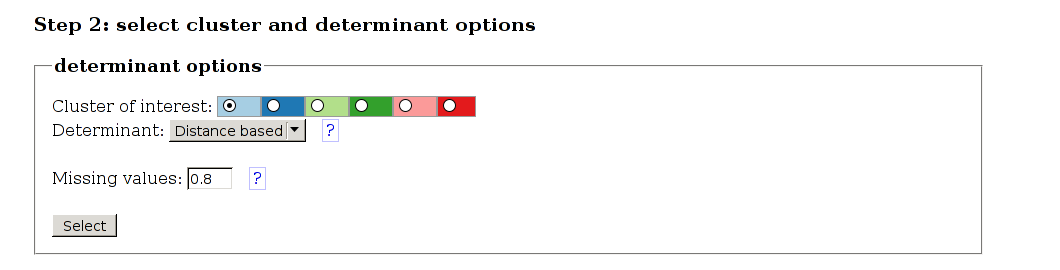
\includegraphics[width=\textwidth]{images/determinant-options.png}
\end{center}

\gabmap{} allows you to choose among two possible determinant methods.
We will cover the default one, labeled `Distance based', can be used 
as long as a distance metric can be calculated between
the sites with respect to linguistic variables. As a result it works
with both categorical (string) and numeric variables. The second one
is particularly suited for categorical data. We will experiment with
the default method here.

The default method calculates average differences between sites within
the cluster of interest and average differences between the sites
inside the cluster and the sites outside the cluster with respect to
all variables. For the string data we are using, a variable is a
certain word or phrase. A linguistic variable is recognized as a
representative variable for the cluster, if the average difference
within the cluster is low and the average difference between cluster
and the rest of the sites is high with respect to this variable.

When you click to \textsc{Select} button after choosing the cluster of
interest and other determinant parameters, a sorted list items are
presented in a list. The list includes three scores for each variable.
The first number is an aggregate score which is the difference of
\emph{between distance} and  \emph{within distance}.  Both of these
values are reported next to the aggregated score. 

For details of these calculations, we refer to the help text available
in \gabmap{} and the referenced papers therein. In informal terms,
\emph{between distance} characterizes how distinct the variable is
between the sites in the cluster and the other sites. \emph{Between
distance}, on the other hand, characterizes how similar the sites in
the cluster are with respect to the variable. As a result, we prefer
items with high between difference, and low within difference as
`determinants' of the cluster.

You should note that a score of zero means that the average difference
(within the cluster or between the cluster and the rest of the sites)
is the same as the overall average difference calculated over all
pairs of sites. Hence an item with with within difference zero or
closer is not particularly uniform among the sites within the cluster.
Similarly, an item with zero or close to zero between difference value
is not distinctive for the cluster.


\begin{Exercise}
Using default clustering and cluster determinant options, find the items 
with the lowest within difference and the highest between difference.  
If you like to see all items at once in a list, or export it to a 
spreadsheet application, you can use the link \emph{Download as list}.
\end{Exercise}

If you want to investigate the further differences with respect to an
item further, you can choose the item in the list, and click
\textsc{Select item}. This will present you with a difference map
similar to link maps in \emph{Statistics and difference maps} tool.
The sites within the cluster are marked with black dots. If you hover
your mouse over a site, the pronunciations recorded in the site is
displayed together with its name.

\begin{Exercise}
Select the item with the highest aggregate score, and examine the map.
Do the scores agree with what you see in the map?
\end{Exercise}

Furthermore, the pronunciations of the item that are observed within
the cluster and outside the cluster are listed below the map. The
numbers next to the pronunciation are the number of times a
pronunciation is observed in the cluster and the total number of times
the pronunciation is observed anywhere. If you select a set of
pronunciations and click \textsc{Show distribution map}, you are
presented with a distribution map similar to the other tools available
in \gabmap{}.

\begin{Exercise}
With the default options, you get the item \emph{shades} with a very
low score of -1.01. A negative score means that the item is more
varied within the cluster compared to the variation between the
cluster and other sites. Inspect the difference and distribution maps
for this item. Can you explain the reason for this very low score?
\end{Exercise}

The option `Missing values' in cluster determinant options controls
what to do when distances between individual pairs of sites cannot be
calculated with respect a particular item due to missing data. If the
missing values are greater than the chosen ratio, the cluster
determinant score is not reported. 

\begin{Exercise}
Default option for `\emph{Missing values}' is 0.8, which means the scores
will be calculated even if 80\% of the pairwise distances cannot be
calculated due to missing values. Recalculate the cluster determinants
with the Missing values option set such that we do not calculate the
score only if all pairwise differences can be calculated. How many
items are left out because of this setting?
\end{Exercise}

\begin{Exercise}
After above exercise, the lowest scoring items should be \emph{six}
and \emph{from the south}. Inspect both elements using difference maps
and distribution maps and explain the reasons these items have
negative scores.
\end{Exercise}

\end{document}
